\documentclass[letterpaper]{sig-alternate}
%\documentclass[10pt]{sensys-proc}

\setlength{\paperheight}{11in}
\setlength{\paperwidth}{8.5in}
\usepackage[
  pass,% keep layout unchanged 
  % showframe,% show the layout
]{geometry}

%\usepackage{draftwatermark}
%\usepackage{epsfig}
%\usepackage{epstopdf}
%\usepackage{afterpage}
\usepackage{balance}
%\usepackage{fancyvrb}
%\usepackage[utf8]{inputenc}
%\usepackage[usenames,dvipsnames]{xcolor}
\usepackage{verbatim}
\usepackage{xspace}
%\usepackage{amssymb}
%\usepackage{amsmath}
%\usepackage{fancyvrb}
%\usepackage{booktabs}
%\usepackage{colortbl}
%\usepackage{tabularx}
%\usepackage{multirow}
\usepackage{color}
\usepackage{xcolor,colortbl}
%\usepackage{hyperref}    % Creates hyperlinks from ref/cite 
%\hypersetup{pdfstartview=FitH}
\usepackage{graphicx}
\usepackage{url}

\definecolor{light}{gray}{0.97}
\definecolor{dark}{gray}{0.30}
%\definecolor{light}{rgb}{.90,.90,.90}
\definecolor{darkgreen}{rgb}{0,.50,0}
\definecolor{darkblue}{rgb}{0,0,.50}
\definecolor{darkred}{rgb}{.50,0,0}
\definecolor{darkpur}{rgb}{.50,0,.50}

\usepackage{listings}
%\usepackage{textcomp}
\lstset{
%columns=fullflexible,
%basicstyle=\ttfamily,
escapeinside={||},
mathescape=true,
    language=C, % choose the language of the code
    basicstyle=\fontfamily{pcr}\selectfont\small\color{black},
    keywordstyle=\color{black}\bfseries, % style for keywords
    numbers=none, % where to put the line-numbers
    numberstyle=\tiny, % the size of the fonts that are used for the line-numbers
    backgroundcolor=\color{light},
    %showspaces=false, % show spaces adding particular underscores
    %showstringspaces=false, % underline spaces within strings
    showtabs=false, % show tabs within strings adding particular underscores
    %frame=single, % adds a frame around the code
    tabsize=2, % sets default tabsize to 2 spaces
    %rulesepcolor=\color{gray}
    captionpos=t, % sets the caption-position to bottom
    breaklines=false, % sets automatic line breaking
    %breakatwhitespace=false,
    numbersep=2em,
    emph={par,or,do,end,loop,await,emit,input,event,call,with,command,%
          var,and,then,else,native,return,pure,safe,nohold,finalize},
    emphstyle={\bfseries},
    %commentstyle=\color{dark},
    commentstyle=\color{dark}\scriptsize,
    %xleftmargin=20pt,
    %xrightmargin=20pt,
    framesep=20pt,
    %upquote=true,
    %aboveskip={1.5\baselineskip},
}

\newcommand{\footnoteremember}[2]{%
\footnote{#2}%
\newcounter{#1}%
\setcounter{#1}{\value{footnote}}%
}
\newcommand{\footnoterecall}[1]{%
\footnotemark[\value{#1}]%
}

%\renewcommand{\arraystretch}{1.2} % Space out rows in tables

\setlength\paperheight {11in}
\setlength\paperwidth {8.5in}

% No space between bibliography items:
\let\oldthebibliography=\thebibliography
  \let\endoldthebibliography=\endthebibliography
  \renewenvironment{thebibliography}[1]{%
    \begin{oldthebibliography}{#1}%
      \setlength{\parskip}{0ex}%
      \setlength{\itemsep}{0ex}%
  }%
  {%
    \end{oldthebibliography}%
  }
\setlength{\parindent}{5mm}

\newcommand{\compresslist}{
	\setlength{\itemsep}{1pt}
	\setlength{\parskip}{0pt}
	\setlength{\parsep}{0pt}
}

\newenvironment{itemize*}%
  {\begin{itemize}%
    \setlength{\itemsep}{0pt}%
    \setlength{\parskip}{0pt}}%
  {\end{itemize}}
\usepackage{enumitem}
\setlist{nolistsep}

%\relpenalty=9999
%\binoppenalty=9999

\newcommand{\code}[1] {{\small{\texttt{#1}}}}
\newcommand{\Code}[1] {\texttt{#1}}
\newcommand{\CEU}{\textsc{C\'{e}u}\xspace}

\def\sharedaffiliation{%
\end{tabular}
\begin{tabular}{c}
}

%\author{
%Paper \#42
%}

\numberofauthors{5}
\author{
    \alignauthor Francisco Sant'Anna        \\
        \email{fsantanna@inf.puc-rio.br}
    \alignauthor Noemi Rodriguez            \\
        \email{noemi@inf.puc-rio.br}
    \alignauthor Roberto Ierusalimschy      \\
        \email{roberto@inf.puc-rio.br}
    \sharedaffiliation
    \affaddr{Departamento de Inform\'atica --
             PUC-Rio, Brazil}
\vspace{0.5cm}
\and
    \alignauthor Olaf Landsiedel \\
         \email{olafl@chalmers.se}
    \alignauthor Philippas Tsigas \\
         \email{tsigas@chalmers.se}
    \sharedaffiliation
    \affaddr{Computer Science and Engineering --
             Chalmers University of Technology, Sweden}
}

\begin{comment}
\numberofauthors{5}
\author{
    \alignauthor XXXXXXXX XXXXXXXX        \\
        \email{xxxxxxxx@xxxxxxxxxxxx}
    \alignauthor XXXXXXXX XXXXXXXX            \\
        \email{xxxxxxxx@xxxxxxxxxxxx}
    \alignauthor XXXXXXXX XXXXXXXX      \\
        \email{xxxxxxxx@xxxxxxxxxxxx}
    \sharedaffiliation
    \affaddr{XXXXXXXX XXXXXXXX XXXXXXXX --
             XXXXXXXX XXXXXXXX, XXXXXXXX}
\vspace{0.5cm}
\and
    \alignauthor XXXXXXXX XXXXXXXX \\
         \email{xxxxxxxx@xxxxxxxxxxxx}
    \alignauthor XXXXXXXX XXXXXXXX \\
         \email{xxxxxxxx@xxxxxxxxxxxx}
    \sharedaffiliation
    \affaddr{XXXXXXXX XXXXXXXX XXXXXXXX --
             XXXXXXXX XXXXXXXX, XXXXXXXX}
}
\end{comment}

%\title{Safe Concurrent Abstractions for Wireless Sensor Networks}
%\title{Safe Synchronous Abstractions for Wireless Sensor Networks}
\title{Safe System-level Concurrency on Resource-Constrained Nodes}

%\crdata{978-1-4503-2027-6} %/13/11…$15.00.
%\crdata{978-1-4503-1169-4}
%\conferenceinfo{SenSys'13,} {November 11--15, 2013, Rome, Italy.}
%\CopyrightYear{2013}

%Copyright is held by the owner/author(s). Publication rights licensed to ACM.
%http://dx.doi.org/10.1145/2517351.2517360

% TeXSupport
\makeatletter
\def\doi#1{\gdef\@doi{#1}}\def\@doi{}
\toappear{\the\boilerplate\par{\confname{\the\conf}} \the\confinfo\par \the\copyrightetc.\ifx\@doi\@empty\else\par\@doi.\fi}
%%
\newfont{\mycrnotice}{ptmr8t at 7pt}
\newfont{\myconfname}{ptmri8t at 7pt}
\let\crnotice\mycrnotice%
\let\confname\myconfname%
\makeatother

%
% --- Author Metadata here ---
% Permission Statement
\permission{
Permission to make digital or hard copies of all or part of this work for 
personal or classroom use is granted without fee provided that copies are not 
made or distributed for profit or commercial advantage and that copies bear 
this notice and the full citation on the first page. Copyrights for components 
of this work owned by others than the author(s) must be honored.  Abstracting 
with credit is permitted. To copy otherwise, or republish, to post on servers 
or to redistribute to lists, requires prior specific permission and/or a fee.  
Request permissions from Permissions@acm.org.}

% Conference Information
\conferenceinfo{SenSys'13,}{November 11-15, 2013, Rome, Italy.\\
Copyright is held by the owner/author(s). Publication rights licensed to ACM.}
\CopyrightYear{2013}
\crdata{978-1-4503-2027-6/13/11}

% DOI
\doi{http://dx.doi.org/10.1145/2517351.2517360}
%


\begin{document}

\maketitle

% TODO: CTP / DRIP ROM reduction
% motivation timers
% category for related papers
% ref na tabela related
% figuras que explicam experimentos
% PCTS na mao na tabela de eval (+/-)

\begin{abstract}

% TODO: split 2 sents.
Despite the continuous research to facilitate WSNs development, most safety 
analysis and mitigation efforts in concurrency are still left to developers, 
who must manage synchronization and shared memory explicitly.
% among activities explicitly.
%
In this paper, we present a system language that ensures safe concurrency by 
handling threats at compile time, rather than at runtime.
%
Based on the synchronous programming model, our design allows for a simple 
reasoning about concurrency that enables compile-time analysis resulting in 
deterministic and memory-safe programs.
%
As a trade-off, our design imposes limitations on the language expressiveness, 
such as doing computationally-intensive operations and meeting hard real-time 
responsiveness.
% defining, doing, executing, describing
%
To show that the achieved expressiveness and responsiveness is sufficient for a 
wide range of WSN applications, we implement widespread network protocols and 
the CC2420 radio driver.
%
The implementations show a reduction in source code size, with a penalty of 
memory increase below 10\% in comparison to \emph{nesC}.
%
Overall, we ensure safety properties for programs relying on high-level control 
abstractions that also lead to concise and readable code.
% in terms of total ROM/RAM.
%, and a negligible increase in CPU usage.

\end{abstract}

% A category with the (minimum) three required fields
%\category{H.4}{Information Systems Applications}{Miscellaneous}
%A category including the fourth, optional field follows...
%\category{D.2.8}{Software Engineering}{Metrics}[complexity measures, 
%performance measures]

%\terms{Delphi theory}

%\keywords{ACM proceedings, \LaTeX, text tagging}

%\category{D.3}{Programming Languages}{General}
%\category{D.3.3}{Programming Languages}{Language Constructs and Features}

%\terms{Design, Languages, Reliability}

%\keywords{Concurrency, Determinism, Safety, Static Analysis, Synchronous, 
%Wireless Sensor Networks}

\section{Introduction}
\label{sec.intro}

\begin{comment}
System-level development for WSNs basically consists of abstracting access to 
the hardware and designing specially tweaked network protocols to be further 
integrated as services in higher-level applications or macro-programming 
systems~\cite{wsn.state_of_art,wsn.tos,wsn.survey}.
%The external environment plays an important, as it interacts with applications 
%permanently (and concurrently) by issuing events that represent expiring 
%timers, messages arrivals, sensor readings, etc.

Our design is first compromised with the main principles that govern WSN 
development: \emph{resource minimization} and \emph{bug prevention}, as defined 
by Levis~\cite{wsn.decade}.

\end{comment}

System-level development for Wireless Sensor Networks (WSNs) commonly follows 
one of three major programming models: \emph{event-driven}, 
\emph{multi-threaded}, or \emph{synchronous}.
%
In event-driven programming \cite{wsn.tos,wsn.contiki}, each external event can 
be associated with a short-lived function callback to handle a reaction to the 
environment.
This model is efficient,
% for the severe resource constraints of WSNs,
but is known to be difficult to 
program~\cite{sync_async.cooperative,wsn.protothreads}.
%
Multi-threaded systems emerged as an alternative in WSNs, providing traditional 
structured programming in multiple lines of 
execution~\cite{wsn.protothreads,wsn.mantisos}.
However, the development process still requires manual synchronization and 
bookkeeping of threads~\cite{sync_async.threadsproblems}.
%(e.g. create, start, and rejoin)
%
Synchronous languages~\cite{rp.twelve} have also been adapted to WSNs and offer 
higher-level compositions of activities with a step-by-step execution, 
considerably reducing programming efforts~\cite{wsn.sol,wsn.osm}.

Despite the increase in development productivity, WSN system languages still 
fail to ensure static safety properties for concurrent programs.
%
However, given the difficulty in debugging WSN applications, it is paramount to 
push as many safety guarantees to compile time as possible~\cite{wsn.decade}.
%
Shared-memory concurrency is an example of a widely adopted mechanism that 
typically relies on runtime safety primitives only.
For instance, current WSN languages ensure atomic memory access either through 
runtime barriers, such as mutexes and 
locks~\cite{wsn.mantisos,wsn.tinythreads}, or by adopting cooperative 
scheduling which also requires explicit yield points in the 
code~\cite{wsn.sol,wsn.protothreads}.
%Requiring explicit synchronization primitives lead to potential safety 
%hazards~\cite{sync_async.threadsproblems}.
%Enforcing cooperative scheduling is no less questionable, as it assumes that 
%\emph{all} accesses are dangerous.
In either case, there are no additional static guarantees or warnings about 
unsafe memory accesses.
%The bottom line is that existing languages cannot detect and enforce atomicity 
%only when they are required.

\begin{figure*}[!t]
%\rule{8.5cm}{0.37pt}
\begin{minipage}[t]{0.27\linewidth}
\begin{lstlisting}[title=\emph{/* nesC */}]
|{\color{darkgreen}\textbf{event void} Boot.booted () \{}|
  |{\color{darkblue}\textbf{call} T1.start(0)}|
  |{\color{darkpur}\textbf{call} T2.start(60000)}|
|{\color{darkgreen}\}}|
|{\color{darkblue}\textbf{event void} T1.fired () \{}|
  |{\color{darkblue}\textbf{static int} on = 0;}|
  |{\color{darkblue}\textbf{if} (on) \{}|
    |{\color{darkblue}\textbf{call} Leds.led0Off();}|
    |{\color{darkblue}\textbf{call} T1.start(1000);}|
  |{\color{darkblue}\} \textbf{else} \{}|
    |{\color{darkblue}\textbf{call} Leds.led0On();}|
    |{\color{darkblue}\textbf{call} T1.start(2000);}|
  |{\color{darkblue}\}}|
  |{\color{darkblue}on = !on;}|
|{\color{darkblue}\}}|
|{\color{darkpur}\textbf{event void} T2.fired() \{}|
  |{\color{darkred}\textbf{call} T1.cancel();}|
  |{\color{darkred}\textbf{call} Leds.led0Off();}|
  |{\color{darkred}<...> // CONTINUE}|
}

\end{lstlisting}
\end{minipage}
%
\hfill \vrule \hfill
\hspace{0.0cm}
%
\begin{minipage}[t]{0.30\linewidth}
%\fbox{
\begin{lstlisting}[title=\emph{/* Protothreads */}]
|{\color{darkgreen}\textbf{int} main () \{}|
  |{\color{darkblue}\textbf{PT\_INIT(\&blink);}}|
  |{\color{darkpur}timer\_set(\&timeout, 60000);}|
  |{\color{darkred}\textbf{while} (}|
    |{\color{darkred}\textbf{PT\_SCHEDULE}(blink()) \&\&}|
    |{\color{darkred}!timer\_expired(timeout)}|
  |{\color{darkred});}|
  |{\color{darkred}leds\_off(LEDS\_RED);}|
  |{\color{darkred}<...> // CONTINUE}|
|{\color{darkred}\}}|
|{\color{darkblue}\textbf{PT\_THREAD} blink () \{}|
  |{\color{darkblue}\textbf{while} (1) \{}|
    |{\color{darkblue}leds\_on(LEDS\_RED);}|
    |{\color{darkblue}timer\_set(\&timer, 2000);}|
    |{\color{darkblue}\textbf{PT\_WAIT}(expired(\&timer));}|
    |{\color{darkblue}leds\_off(LEDS\_RED);}|
    |{\color{darkblue}timer\_set(\&timer, 1000);}|
    |{\color{darkblue}\textbf{PT\_WAIT}(expired(\&timer));}|
  |{\color{darkblue}\}}|
|{\color{darkblue}\}}|
\end{lstlisting}
%}
\end{minipage}
%
\hfill \vrule \hfill
\hspace{0.0cm}
%
\begin{minipage}[t]{0.18\linewidth}
%\fbox{
\begin{lstlisting}[title=/* \CEU */]
|\textbf{\color{darkgreen}par/or do}|
  |\textbf{\color{darkblue}loop do}|
    |{\color{darkblue}\_Leds\_led0On();}|
    |{\color{darkblue}await 2s;}|
    |{\color{darkblue}\_Leds\_led0Off();}|
    |{\color{darkblue}await 1s;}|
  |\textbf{\color{darkblue}end}|
|\textbf{\color{darkgreen}with}|
  |{\color{darkpur}\textbf{await} 1min;}|
|\textbf{\color{darkgreen}end}|
|{\color{darkred}\_Leds\_led0Off();}|
|{\color{darkred}<...> // CONTINUE}|
\end{lstlisting}
%}
\end{minipage}
%
\hfill \vrule \hfill
\hspace{0.0cm}
%
\begin{minipage}[t]{0.15\linewidth}
\vspace{30pt}
\centering
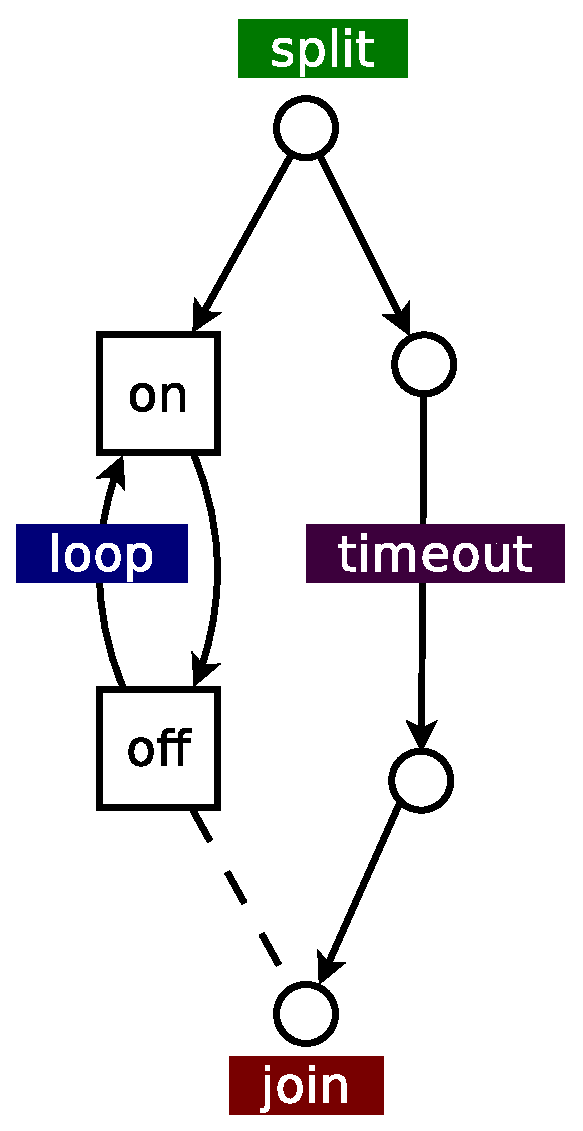
\includegraphics[width=\textwidth]{dia}
\end{minipage}
%
\hspace{0.0cm}
%
\rule{18cm}{0.37pt}
\caption{ ``Blinking LED'' in
    nesC,
    Protothreads,
    and \CEU. %\newline
%{\small
%The colors associate chunks of code with respective actions in the diagram.
%}
\label{lst.all}
}
\end{figure*}

We believe that programming WSNs can benefit from a new language that takes 
concurrency safety as a primary goal, while preserving typical multi-threading 
features that programmers are familiarized with, such as shared memory 
concurrency.
%
In this work, we present the design of \CEU%
\footnote{C\'eu is the Portuguese word for \emph{sky}.},
a synchronous system-level programming language that provides a reliable yet 
powerful set of abstractions for the development of WSN applications.
%
\CEU is based on a small set of control primitives similar to 
Esterel's~\cite{esterel.ieee91}, leading to implementations that more closely 
reflect program specifications.
%
As a main contribution, we propose a static analysis that permeates all 
language mechanisms and detects safety threats at compile time.
This allows \CEU to support safe shared-memory concurrency as well as 
system-level $C$ calls.
%
In addition, we introduce the following new safety mechanisms:
\emph{first-class timers} to ensure precise synchronization among timers in 
parallel (not depending on internal reaction timings);
\emph{finalization blocks} for local pointers going out of scope;
and \emph{stack-based communication} that avoids cyclic dependencies.
%
In contrast with existing synchronous languages, \CEU introduces a stack-based 
execution for internal events which enables a limited but safer form of 
subroutines.
%
Our work focuses on \emph{concurrency safety}, rather than \emph{type 
safety}~\cite{wsn.safety}.%
\footnote{
We consider both safety aspects to be complimentary and orthogonal, i.e., 
type-safety techniques could also be applied to \CEU.
}

In order to enable static analysis, programs in \CEU must suffer some 
limitations.
Computations that run in unbounded time (e.g., compression, image processing) 
cannot be elegantly implemented~\cite{rp.hypothesis}, and dynamic loading is 
forbidden.
%do not fit the zero-delay reaction hypothesis~\cite{rp.hypothesis}, and
%
%Also, dynamic support in the language, such as memory allocation and dynamic 
%loading, is forbidden.
%
However, we show that \CEU is sufficiently expressive for the context of WSN 
applications.
We successfully implemented the \emph{CC2420} radio driver, and the 
\emph{DRIP}, \emph{SRP}, and \emph{CTP} network protocols~\cite{wsn.teps} in 
\CEU.
In comparison to \emph{nesC}~\cite{wsn.nesc}, the implementations reduced the 
number of source code tokens by 25\%, with an increase in ROM and RAM below 
10\%.
%The radio driver also shows a responsiveness equivalent to \emph{nesC} in most 
%scenarios.

The rest of the paper is organized as follows:
Section~\ref{sec.overview} gives an overview on how different programming 
models used in WSNs can express typical control patterns.
Section~\ref{sec.ceu} details the design of \CEU, motivating and discussing the
safety aspects of each relevant language feature.
Section~\ref{sec.eval} evaluates the implementation of the network protocols in 
\CEU and compares some of its aspects with \emph{nesC} (e.g. memory usage and 
tokens count).
We also evaluate the responsiveness of the radio driver written in \CEU, 
showing extreme high-load conditions in which the disciplined synchronous 
execution of our model may not be suitable.
Section~\ref{sec.related} discusses related work to \CEU.
Section~\ref{sec.conclusion} concludes the paper and makes final remarks.

\section{Overview of Programming Models}
\label{sec.overview}

WSN applications must handle a multitude of concurrent events, such as timers 
and packet transmissions.
Although they may seem random and unrelated for an external observer, a
program must logically keep track of them according to its control 
specification.
%
From a control perspective, programs are composed of two main patterns: 
\emph{sequential}, i.e., an activity with two or more sub-activities in 
sequence;
and \emph{parallel}, i.e., unrelated activities that eventually need to 
synchronize.
%
As an example, an application that alternates between sampling a sensor and 
broadcasting its readings has a sequential pattern (with an enclosing loop); 
while including an 1-minute timeout to interrupt an activity denotes a parallel 
pattern.

Figure~\ref{lst.all} presents the three different programming models commonly 
used in WSNs.
It shows the implementations in \emph{nesC}~\cite{wsn.nesc}, 
\emph{Protothreads}\cite{wsn.protothreads}, and \CEU for an application that 
continuously turns on a LED for 2 seconds and off for 1 second.
After 1 minute of activity, the application turns off the LED and proceeds to 
another activity (marked in the code as \code{<...>}).
The diagram on the right of Figure~\ref{lst.all} describes the overall control 
behavior for the application.
The sequential programming pattern is represented by the LED alternating between 
the two states, while the parallel pattern is represented by the 1-minute 
timeout.
% that interrupts the blinking LED.

The first implementation, in \emph{nesC}, which represents the 
\emph{event-driven} model, spawns two timers ``in parallel'' at boot time 
(\code{Boot.booted}): one to make the LED blink and another to wait for 1 
minute.
The callback \code{T1.fired} continuously toggles the LED and resets the timer 
according to the state variable \code{on}.
The callback \code{T2.fired} executes only once, canceling the blinking timer, 
and proceeds to \code{<...>}.
Overall, we argue that this implementation has little structure: the blinking 
loop is not explicit, but instead relies on a static state variable and 
multiple invocations of the same callback.
Furthermore, the timeout handler (\code{T2.fired}) requires specific knowledge 
about how to stop the blinking activity, and the programmer must manually 
terminate it (\code{T1.cancel()}).

The second implementation, in \emph{Protothreads}, which represents the 
\emph{multi-threaded} model, uses a dedicated thread to make the LED blink in a 
loop.
This brings more structure to the solution.
The main thread also helps a reader to identify the overall sequence of the 
program, which is not easily identifiable in the event-driven implementation 
without tracking the dependencies among callbacks.
However, it still requires much bookkeeping for initializing, scheduling and 
rejoining the blinking thread after the timeout (inside the \code{while} 
condition).

% ASYNC MT?

The third implementation, in \CEU, which represents the \emph{synchronous 
model}, uses a \code{par/or} construct to run the two activities in parallel:
an endless loop to blink the LED, and a single statement that waits for 1 
minute before terminating.
The \code{par/or} stands for \emph{parallel-or} and rejoins automatically when 
any of its lines of execution terminates.
(\CEU also supports \code{par/and} compositions, which rejoin when \emph{all} 
spawned lines of execution terminate.)
%
We argue that the hierarchical structure of \CEU more closely reflects the 
control diagram and ties the two activities together, implying that
(a) they can only exist together;
(b) they always start together;
(c) they always terminate together.
%
Besides the arguably cleaner syntax, the additional control-flow information 
that can be inferred from the program is the base for all features and safety 
guarantees introduced by \CEU.

% TODO
%The challenge is how to provide a design that embraces/xxx safety/determinism, 
%specially considering pointers

%\afterpage{clearpage}
\section{The Design of C\'eu}
\label{sec.ceu}

\begin{figure}[t]
\begin{lstlisting}%[backgroundcolor=\color{white}]

// DECLARATIONS
input <type> <id>;      // external event
event <type> <id>;      // internal event
var   <type> <id>;      // variable

// EVENT HANDLING
await <id>;             // awaits event
emit  <id>;             // emits  event

// COMPOUND STATEMENTS
<...> ; <...> ;         // sequence
if <...> then <...>     // conditional
         else <...> end
loop do <...> end       // repetition
    break               //   (escape loop)
finalize <...>          // finalization
    with <...> end

// PARALLEL COMPOSITIONS
par/and do <...>        // rejoins on both sides
      with <...> end
par/or do  <...>        // rejoins on any side
      with <...> end
par do <...>            // never rejoins
  with <...> end

// C INTEGRATION
_f();                   // C call (prefix `_')
native do <...> end     // block of native code
pure <id>;              // "pure" annotation
safe <id> with <id>;    // "safe" annotation
\end{lstlisting}
\rule{8.5cm}{0.37pt}
\caption{ Syntax of \CEU.\newline
{\small %\textmd{
}%}
\label{lst.syntax}
}
\end{figure}

\CEU is a concurrent language in which multiple lines of execution---known as 
\emph{trails}---continuously react to input events from the environment.
Waiting for an event halts the running trail until that event occurs.
The environment broadcasts an occurring event to all active trails, which share 
a single global time reference (the event itself).
%
%\subsection{Parallel syntactic compositions}
%\label{sec.ceu.par}
%
The fundamental distinction between \CEU and prevailing multi-threaded designs 
is the way threads are combined in programs.
\CEU provides Esterel-like syntactic hierarchical compositions, while most 
multi-threaded systems typically only support top-level definitions for 
threads.
Figure~\ref{lst.syntax} shows a compact reference of \CEU, which helps to 
follow the examples in this chapter.
%\CEU distinguishes itself from Esterel by its tight integration with $C$ and 
%support for shared memory, which also demands an effective safety analysis 
%permeating (and affecting) all language features.

As an introductory example, the code in Figure~\ref{lst.radio} is extracted 
from our implementation of the \emph{CC2420} radio driver~\cite{wsn.teps} and 
uses a \code{par/or} to control the start/stop behavior of the radio.
The input events \code{CC2420\_START} and \code{CC2420\_STOP} (line 1) 
represent the external interface of the driver with a client application (e.g.  
a protocol).
The driver enters the top-level loop and awaits the starting event (line 3);
upon request, the driver spawns two other trails:
one to await the stopping event (line 5),
and another to actually receive radio messages in a loop (collapsed in line 9).
%
As compositions can be nested, the receiving loop can be as complex as needed 
and contain other loops and parallel constructs.
However, once the client requests to stop the driver, the trail in line 5 
awakes and terminates, also terminating the \code{par/or} which aborts the 
receiving loop and proceeds to the statement in sequence.
In this case, the top-level loop restarts, waiting for the next request to 
start (line 3, again).

\begin{figure}[t]
\begin{lstlisting}[numbers=left,xleftmargin=2.5em]
input void CC2420_START, CC2420_STOP;
loop do
    await CC2420_START;
    par/or do
        await CC2420_STOP;
    with
        // loop with other nested trails
        // to receive radio packets
        <...>
    end
end
\end{lstlisting}
\rule{8.5cm}{0.37pt}
\caption{ Start/stop behavior for the radio driver.\newline
{\small %\textmd{
The occurrence of \code{CC2420\_STOP} (line 5) seamlessly aborts the receiving 
loop (collapsed in line 9) and resets the driver to wait for the next 
\code{CC2420\_START} (line 3).
}%}
\label{lst.radio}
}
\end{figure}

The \code{par/or} construct is regarded as an \emph{orthogonal preemption 
primitive}~\cite{esterel.preemption} because the two sides in the composition 
need not to be tweaked with synchronization primitives or state variables in
order to affect each other.
In contrast, it is known that traditional (asynchronous) multi-threaded 
languages cannot express thread abortion 
safely~\cite{esterel.preemption,sync_async.threadsstop}.

\begin{comment}
The same start/stop control pattern for the radio driver appears in all ported 
network protocols presented in Section~\ref{sec.eval}.
In practical terms, parallel compositions eliminated all state variables in our 
ports, not only those related to split-phase 
operations~\cite{wsn.protothreads}.
\end{comment}

\subsection{Deterministic and Bounded Execution}
\label{sec.ceu.det}

% TODO: motivate?

\CEU is grounded on a precise definition of time as a discrete sequence of 
external input events:
% \footnote{We use the terms \emph{external input event}, \emph{external event}, 
%and \emph{input event} interchangeably.}
a sequence because only a single input event is handled at a time; discrete 
because reactions to events are guaranteed to execute in bounded time (to be 
discussed further).
The execution model for a program in \CEU is as follows:

\begin{enumerate}
\item The program initiates the ``boot reaction'' in a single trail.
\item Active trails execute until they await or terminate.
      This step is named a \emph{reaction chain}, and always runs in bounded 
      time.
\item The program goes idle and the environment takes control.
\item On the occurrence of a new external input event, the environment awakes 
      \emph{all} trails awaiting that event.
      It then goes to step 2.
\end{enumerate}

% TODO
The synchronous execution model of \CEU is based on the hypothesis that 
internal reactions run \emph{infinitely faster} in comparison to the rate of 
external events~\cite{rp.hypothesis}.
Conceptually, a program takes no time on step 2 and is always idle on step 3.
In practice, if a new external input event occurs while a reaction chain is 
running (step 2), it is enqueued to run in the next reaction.
%, because reaction chains must run to completion.
%
% TODO: a similar approach is taken in \cite{...}
%
When multiple trails are active at a time (i.e. awaking on the same event), 
\CEU schedules them in the order they appear in the program source code.
This policy is somewhat arbitrary, but provides a priority scheme for trails, 
and also ensures deterministic and reproducible execution for programs, which 
is important for simulation purposes.
A reaction chain may also contain emissions and reactions to internal events, 
which are presented in Section~\ref{sec.ceu.ints}.

The blinking LED of Figure~\ref{lst.all} in \CEU illustrates how the 
synchronous model leads to a simpler reasoning about concurrency aspects in 
comparison to the other implementations.
As reaction times are assumed to be instantaneous, the blinking loop takes 
exactly $2+1$ seconds.
Hence, after 20 iterations, the accumulated time becomes 1 minute and the loop 
terminates concurrently with the 1-minute timeout in parallel.
Given that the loop appears first, it will restart and turn on the LED for the 
last time.
Then, the 1-minute timeout is scheduled, aborts the whole \code{par/or}, and 
turns off the LED.
%
This reasoning is actually reproducible in practice, and the LED will light on 
exactly 21 times for every single execution of this program.
First-class timers are discussed in more depth in 
Section~\ref{sec.ceu.wclocks}.
%
Note that this static control inference cannot be easily extracted from the 
other implementations of Figure~\ref{lst.all}, specially considering the 
presence of two different timers.

The behavior for the LED timeout just described denotes a \emph{weak abortion}, 
because the blinking trail had the chance to execute for one last time.
By inverting the two trails, the \code{par/or} would terminate immediately, and 
the blinking trail would not execute, denoting a \emph{strong 
abortion}~\cite{esterel.preemption}.
%
\CEU not only provides means to choose between weak and strong abortion, but 
also detects the two conflicting possibilities and issues a warning at compile 
time (to be discussed in Section~\ref{sec.ceu.shared}).

Reaction chains should run in bounded time to guarantee that programs are 
responsive and can handle upcoming input events from the environment.
Similarly to Esterel~\cite{esterel.ieee91}, \CEU requires that each possible 
path in a loop body contains at least one \code{await} or \code{break} 
statement, thus ensuring that loops never run in unbounded time.
%
Consider the examples that follow:

\nopagebreak
\noindent
\begin{minipage}[t]{0.45\linewidth}
\begin{lstlisting}
loop do
    if <cond> then
        await A;
    end
end
\end{lstlisting}
\end{minipage}
%
\begin{minipage}[t]{0.45\linewidth}
\begin{lstlisting}
loop do
    if <cond> then
        await A;
    else
        break;
    end
end
\end{lstlisting}
\end{minipage}

The first example is refused at compile time, because the \code{if} true branch 
may never execute, resulting in a \emph{tight loop} (i.e., an infinite loop 
that does not await).
The second variation is accepted, because for every iteration, the loop either 
breaks or awaits.

% TTT: unrestrict-ed
Enforcing bounded execution makes \CEU inappropriate for algorithmic-intensive 
applications that require unrestrict-ed loops (e.g., cryptography, image 
processing).
However, \CEU is designed for control-intensive applications and we believe 
this is a reasonable price to pay in order to achieve higher reliability.

% TODO: pause

\newpage % TTT

\subsection{Shared-memory Concurrency}
\label{sec.ceu.shared}

WSN applications make extensive use of shared memory, such as for handling 
memory pools, message queues, routing tables, etc.
Hence, an important goal of \CEU is to ensure a reliable execution for 
concurrent programs that share memory.
%
Concurrency in \CEU is characterized when two or more trail segments in 
parallel execute during the same reaction chain.
A trail segment is a sequence of statements followed by an \code{await} (or 
termination).

In the first example that follows, the two assignments to \code{x} run 
concurrently, because both trail segments are spawned during the same reaction 
chain.
However, in the second example, the assignments to \code{y} are never 
concurrent, because \code{A} and \code{B} are different external events and the 
respective segments can never execute during the same reaction chain:

\nopagebreak
\noindent
\begin{minipage}[t]{0.45\linewidth}
\begin{lstlisting}
var int x=1;
par/and do
    x = x + 1;
with
    x = x * 2;
end
\end{lstlisting}
\end{minipage}
%
\begin{minipage}[t]{0.45\linewidth}
\begin{lstlisting}
input void A, B;
var int y=0;
par/and do
    await A;
    y = y + 1;
with
    await B;
    y = y * 2;
end
\end{lstlisting}
\end{minipage}

Note that although the variable \code{x} is accessed concurrently in the first 
example, the assignments are both atomic and deterministic%
\footnote{
Remember from Section~\ref{sec.ceu.det} that trails are scheduled in the order 
they appear and run to completion (i.e., until they await or terminate).
}: the final value of \code{x} is always $4$ (i.e. {\small$(1+1)*2)$}).
%
However, programs with concurrent accesses to shared memory are suspicious, 
because an apparently innocuous reordering of trails modifies the semantics of 
the program; for instance, the previous example would yield $3$ with the trails 
reordered, i.e., {\small$(1*2+1)$}.

%Moreover, \CEU also supports pointers, which are required for low-level 
%manipulation (e.g., accessing buffers from device drivers).

We developed a compile-time temporal analysis for \CEU in order to detect 
concurrent accesses to shared variables, as follows:
\emph{if a variable is written in a trail segment, then a concurrent trail 
segment cannot read or write to that variable, nor dereference a pointer of 
that variable type.}
An analogous policy is applied for pointers \emph{vs} variables and pointers 
\emph{vs} pointers.
The algorithm for the analysis holds the set of all events in preceding 
\code{await} statements for each variable access.
Then, the sets for all accesses in parallel trails are compared to assert that 
no events are shared among them.
Otherwise the compiler warns about the suspicious accesses.

Consider the three examples in Figure~\ref{lst.det}.
The first code is detected as suspicious, because the assignments to \code{x} 
and \code{p} (lines 11 and 14) may be concurrent in a reaction to \code{A} 
(lines 6 and 13);
%
In the second code, although two of the assignments to \code{y} occur in 
reactions to \code{A} (lines 4-5 and 10-11), they are not in parallel trails 
and, hence, are safe.
%Note that the assignment in reaction to \code{B} (line 8) is safe given that 
%reactions to different events cannot overlap (due to the single-event rule).
%
The third code illustrates a false positive in our algorithm: the assignments 
to \code{z} in parallel can only occur in different reactions to \code{A} 
(lines 5 and 9), as the second assignment awaits two occurrences of \code{A}, 
while the first trail assigns and terminates in the first occurrence.

\begin{figure}[t]
\begin{minipage}[t]{0.40\linewidth}
\begin{lstlisting}[numbers=left,xleftmargin=2.5em]
input void A;
var int x;
var int* p;
par/or do
 loop do
   await A;
   if <cnd> then
     break;
   end
 end
 x = 1;
with
 await A;
 *p = 2;
end

\end{lstlisting}
\end{minipage}
%
%
\begin{minipage}[t]{0.31\linewidth}
\begin{lstlisting}
input void A,B;
var int y;
par/or do
  await A;
  y = 1;
with
  await B;
  y = 2;
end
await A;
y = 3;

\end{lstlisting}
\end{minipage}
%
%
\begin{minipage}[t]{0.27\linewidth}
\begin{lstlisting}
input void A;
var int z;
par/and do
  await A;
  z = 1;
with
  await A;
  await A;
  z = 2;
end
\end{lstlisting}
\end{minipage}
%
\rule{8.5cm}{0.37pt}
\caption{ Automatic detection for concurrent accesses to shared memory. \newline
{\small %\textmd{
The first example is suspicious because \code{x} and \code{p} can be accessed 
concurrently (lines 11 and 14).
The second example is safe because accesses to \code{y} can only occur in 
sequence.
The third example illustrates a false positive in our algorithm.
}%}
\label{lst.det}
}
\end{figure}

Conflicting weak and strong abortions, as introduced in 
Section~\ref{sec.ceu.det}, are also detected with the proposed algorithm.
Besides accesses to variables, the algorithm also keeps track of trail 
terminations inside a \code{par/or}, issuing a warning when they can occur 
concurrently.
This way, the programmer can be aware about the conflict existence and choose
between weak or strong abortion.

The proposed static analysis is only possible due to the uniqueness of external 
events within reactions and support for syntactic compositions, which provide 
precise information about the flow of trails (i.e., which run in parallel and 
which are guaranteed to be in sequence).
Such precious information cannot be inferred when the program relies on state 
variables to handle control, as typically occurs in event-driven systems.

We also implemented an alternative algorithm that converts a \CEU program into 
a deterministic finite automata.
The resulting DFA represents all possible points a program can reach during 
runtime and, hence, eliminates all false positives in the static analysis.
However, the algorithm is exponential and may be impractical in some 
situations.
%
That being said, the simpler static analysis does not detect false positives in 
any of the
implementations to be presented in Section~\ref{sec.eval} and executes in 
negligible time, suggesting that the algorithm is practical.

\subsection{Integration with C}
\label{sec.ceu.c}

Most existing operating systems and libraries for WSNs are based on $C$, given 
its omnipresence and level of portability across embedded platforms.
Therefore, it is fundamental that programs in \CEU have access to all 
functionality the underlying platform already provides.

In \CEU, any identifier prefixed with an underscore is repassed \emph{as is} to 
the $C$ compiler that generates the final binary.
Therefore, access to $C$ is seamless and, more importantly, easily trackable.
%
\CEU also supports \emph{native~blocks} to define new symbols in $C$, as 
Figure~\ref{lst.c} illustrates.
Code inside ``\code{native~do~...~end}'' is also repassed to the $C$ compiler 
for the final generation phase.
%Only global definitions are allowed inside $C$ blocks.
As \CEU{} mimics the type system of $C$, values can be easily passed back and 
forth between the languages.

% TODO: real example?
\begin{figure}[t]
\begin{lstlisting}[numbers=left,xleftmargin=2em]
native do
    #include <assert.h>
    int I = 0;
    int inc (int i) {
        return I+i;
    }
end
native _assert(), _inc(), _I;
_assert(_inc(_I));
\end{lstlisting}
%
\rule{8.5cm}{0.37pt}
\caption{ A \CEU program with embedded $C$ definitions.
{\small %\textmd{
The globals \code{I} and \code{inc} are defined in the \code{native} block 
(lines 3 and 4-6), and are imported by \CEU in line 8.
$C$ symbols must be prefixed with an underline to be used in \CEU (line 9).
}%}
\label{lst.c}
}
\end{figure}

$C$ calls are fully integrated with the static analysis presented in
Section~\ref{sec.ceu.shared} and cannot appear in concurrent trails segments, 
because \CEU has no knowledge about their side effects.
Also, passing variables as parameters counts as read accesses to them, while 
passing pointers counts as write accesses to those types (because functions may 
dereference and assign to them).
%
This policy increases considerably the number of false positives in the 
analysis, given that many functions can actually be safely called concurrently.
Therefore, \CEU supports explicit syntactic annotations to relax the policy.
They are illustrated in Figure~\ref{lst.annotations}, and are described as 
follows:

\begin{itemize}
\item The \code{pure} modifier declares a $C$ function that does not cause side 
      effects, allowing it to be called concurrently with any other function in 
the program.
\item The \code{safe} modifier declares a pair of variables or functions that 
      do not affect each other, allowing them to be used concurrently.
\end{itemize}

%The following code illustrates \CEU annotations:
%
% TODO: exs from ports

\begin{figure}[t]
\begin{lstlisting}[numbers=left,xleftmargin=2em]
pure  _abs();          // side-effect free
safe _Leds_led0Toggle with
     _Leds_led1Toggle; // led0 vs led1 is safe
var int* buf1, buf2;   // point to dif. bufs
safe buf1 with buf2;   // buf1 vs buf2 is safe
\end{lstlisting}
\caption{ Annotations for $C$ functions. \newline
{\small %\textmd{
Function \code{abs} is side-effect free and can be concurrent with any other 
function.
The functions \code{\_Leds\_led0Toggle} and \code{\_Leds\_led1Toggle} can 
execute concurrently.
The variables \code{buf1} and \code{buf2} can be accessed concurrently 
(annotations are also applied to variables).
}%}
\label{lst.annotations}
}
\end{figure}

\begin{comment}
TODO

Annotations are typically write-once declarations (when integrating a $C$ 
service for the first time) to be included in actual applications.
Note that the example in Figure~\ref{lst.blink} should include the annotation 
for \code{\_Leds\_led0Toggle} and \code{\_Leds\_led1Toggle} above to be 
compiled correctly.
\end{comment}

\CEU does not extend the bounded execution analysis to $C$ function calls. 
% which are left as responsibility for the programmer.
% TODO: other languages dont as well
On the one hand, $C$ calls must be carefully analyzed in order to keep programs 
responsive.
On the other hand, they also provide means to circumvent the rigor of \CEU in a 
well-marked way (the special underscore syntax).
%
\begin{comment}
This approach is also adopted by Esterel, which supports the \code{call} 
primitive to execute code assumed to be instantaneous in the host 
language~\cite{esterel.primer}.
In \CEU, we take a step further and statically detects when such calls may 
execute concurrently, as discussed in the next section.
\end{comment}
%
Evidently, programs should only resort to $C$ for simple operations that can be 
assumed to be instantaneous, such as non-blocking I/O and \code{struct} 
accessors, but never for control purposes.
% (e.g. interrupt handling).

\subsection{Local Scopes and Finalization}
\label{sec.ceu.fins}

\begin{comment}
Furthermore, system-level development typically involves accesses to the 
underlying platform through $C$ system calls that hold pointers for some time
(e.g. transmission of a message buffer).
Hence, if a local variable goes out of scope and its reference has been 
exposed, a system-level activity may end up with a dangling pointer (i.e. a 
pointer to a freed memory).
\end{comment}

Local declarations for variables bring definitions closer to their use in 
programs, increasing the readability and containment of code.
Another benefit, specially in the context of WSNs, is that blocks in sequence 
can share the same memory space, as they can never be active at the same time.
%
The syntactic compositions of trails allows the \CEU compiler to statically 
allocate and optimize memory usage:
%, as also proposed in other systems~\cite{wsn.osm,wsn.ocram}:
memory for trails in parallel must coexist;
trails that follow rejoin points reuse all memory.

However, the unrestricted use of locals may introduce subtle bugs when dealing 
with pointers and $C$ functions interfacing with device drivers.
Given that hardware components outlive the scope of any local variable, a 
pointer passed as parameter to a system call may be held by a device driver
for longer than the scope of the referred variable, leading to a dangling 
pointer.

The code snippet in Figure~\ref{lst.local} was extracted from our 
implementation of the CTP collection protocol~\cite{wsn.teps}.
The protocol contains a complex control hierarchy in which the trail that sends 
beacon frames (lines 11-16) may be aborted from multiple \code{par/or} trails 
(all collapsed in lines 3, 5, and 9).
%
Now, consider the following behavior:
The sending trail awakes from a beacon timer (line 11).
Then, the local message buffer (line 12) is prepared and passed to the radio 
driver (line 13-15).
While waiting for an acknowledgment from the driver (line 16), the protocol 
receives a request to stop (line 3) that aborts the sending trail and makes the 
local buffer go out of scope.
As the radio driver runs asynchronously and still holds the reference to the 
message (passed in line 15), it may manipulate the dangling pointer.
%
\begin{comment}
The message buffer is declared only where it is required (line 12, in the 6th 
depth-level of the program), but its reference is manipulated by two $TinyOS$ 
global functions:
\code{AMSend\_getPayload} (line 13), which returns the data region of the 
message to be sent; %prepared (collapsed in line 14);
and \code{AMSend\_send} (line 15), which requests the operating system to 
actually send the message.
As the radio driver runs asynchronously and holds the reference to the message 
until it is completely transmitted, the sending trail may be aborted in the 
meantime, resulting in a dangling pointer in the program.
\end{comment}
%
A possible solution is to cancel the message send in all trails that can abort 
the sending trail (through a call to \code{AMSend\_cancel}).
However, this would require expanding the scope of the message buffer, adding a 
state variable to keep track of the sending status, and duplicating the code, 
increasing considerably the complexity of the application.

\begin{figure}[t]
\begin{lstlisting}[numbers=left,xleftmargin=2.5em]
<...>
par/or do
  <...>         // stops the protocol or radio
with
  <...>         // neighbor request
with
  loop do
    par/or do
      <...>   // resends request
    with
      await (dt) ms; // beacon timer expired
      var _message_t msg;
      payload = _AMSend_getPayload(&msg,...);
      <prepare the message>
      _AMSend_send(..., &msg, ...);
      await CTP_ROUTE_RADIO_SENDDONE;
    end
  end
end
\end{lstlisting}
%
\rule{8.5cm}{0.37pt}
\caption{ Unsafe use of local references. \newline
{\small %\textmd{
The period in which the radio driver manipulates the reference to \code{msg} 
passed by \code{\_AMSend\_send} (line 15) may outlive the lifetime of the 
variable scope, leading to an undefined behavior in the program.
}%}
\label{lst.local}
}
\end{figure}

\CEU provides a safer and simpler solution with the following rule:
\emph{$C$ calls that receive pointers require a finalization block to safely 
handle referred variables going out of scope}.
This rule prevents the previous example to compile, forcing the relevant parts 
to be rewritten as shown in Figure~\ref{lst.local.ok}.

\begin{figure}[t]
\begin{lstlisting}[numbers=left,xleftmargin=2.5em]
native nohold _AMSend_getPayload();
    <...>
        var _message_t msg;
        <...>
        finalize
            _AMSend_send(..., &msg, ...);
        with
            _AMSend_cancel(&msg);
        end
   <...>
\end{lstlisting}
%
\rule{8.5cm}{0.37pt}
\caption{ Safe use of local references. \newline
{\small %\textmd{
The call to \code{\_AMSend\_send} is finalized with the call to 
\code{\_AMSend\_cancel}.
%
The call to \code{\_AMSend\_getPayload} does not require finalization because 
it does not hold pointers.
}
\label{lst.local.ok}
}
\end{figure}

First, the \code{nohold} annotation informs the compiler that the referred $C$ 
function does not require finalization code because it does not hold references 
(line 1).
Second, the \code{finalize} construct (lines 5-9) automatically executes the 
\code{with} clause (line 8) when the variable passed as parameter in the 
\code{finalize} clause (line 6) goes out of scope.
Therefore, regardless of how the sending trail is aborted, the finalization 
code politely requests the OS to cancel the ongoing send operation (line 8), 
releasing the reference held by the radio driver.

All network protocols that we implemented in \CEU use this finalization 
mechanism when sending messages.
%
We looked through the TinyOS codebase and realized that among the $349$ calls 
to the \code{AMSend.send} interface, only $49$ have corresponding 
\code{AMSend.cancel} calls.
We verified that many of these \emph{sends} should indeed have matching 
\emph{cancels} because the component provides a \emph{stop} interface for 
clients.
In \emph{nesC}, because message buffers are usually globals, a send that is not 
properly canceled typically results in an extra packet transmission that 
wastes battery.
However, in the presence of dynamic message pools, a misbehaving program can 
change the contents of a (not freed) message that is actually about to be 
transmitted, leading to a subtle bug that is hard to track.

%find . -name "*.nc" | xargs egrep -R "\.send\(|\.send \(" | grep -v command | 
%wc
%=> 349

%find . -name "*.nc" | xargs egrep -R "\.cancel\(|\.cancel \(" | grep -v command | wc
%=> 49

The finalization mechanism is fundamental to preserve the orthogonality of the
\code{par/or} construct, i.e., an aborted trail does not require clean up code 
outside it.

\begin{comment}
% TODO: expand
During the porting process, we identified two potentially harmful system calls 
that require

The send/cancel pattern occurs in all ported applications that use the radio 
for communication evaluated in Section~\ref{sec.eval}.

 that  two dangerous

given that the porting process was straightforward, we believe that the 
\emph{nesC} implementation is free of such ...
However, .
performance degradation
another endorsement

- exception srp queue
we know exactly the place where it occurs
nesC no

* cancel
* timers
* locals

%TODO: LOCALS AND PAR COMPOSITIONS ARE A PERFECT MATCH

As a final consideration, we propose to extend the idea of compositions by 
combining different \emph{applications} together.
In the context of WSNs, it is usually difficult to physically recover motes in 
a deployed network, and by combining multiple applications in a single image, 
we can switch their execution remotely via radio.
The following archetype illustrates this idea:

\nopagebreak
\noindent
\begin{minipage}{\linewidth}
\begin{lstlisting}[numbers=left,xleftmargin=2em]
input int SWITCH;
var int app = 1;
loop do
   par/or do
      app = await SWITCH;
   with
      if app == 1 then
         <CODE for APP1>
      else/if app == 2 then
         <CODE for APP2>
      end
      await FOREVER;
   end
end
\end{lstlisting}
\end{minipage}

The input event \code{SWITCH} (line 1) is used to request application switches 
remotely.%
\footnote{ We are assuming the existence of an hypothetical high-level event 
\code{Switch} that abstracts the radio protocol for requests to change the 
current running application. }
Initially, the code behaves as application $1$ (lines 7-9), but is also waiting 
for a \code{Switch} request in parallel (line 5).
Whenever a new request occurs, the \code{par/or} terminates, aborts the running 
application, and restarts as the requested application.
The \code{await Forever} statement (line 13) ensures that a terminating 
application does not restart itself.

The same idea can be used to \emph{reboot} a mote remotely, in the case of a 
strange behavior in an application.
\end{comment}

\subsection{First-class Timers}
\label{sec.ceu.wclocks}

% TODO: ana

Activities that involve reactions to \emph{wall-clock time}%
\footnote{
By wall-clock time we mean the passage of time from the real world, measured in 
hours, minutes, etc.
}
appear in typical patterns of WSNs, such as timeouts and sensor sampling.
However, support for wall-clock time is somewhat low-level in existing 
languages, usually through timer callbacks or blocking calls with ``sleep''.
%
In any concrete system implementation, however, a requested timeout does not 
expire precisely with zero-delay, a fact that is usually ignored in the 
development process.
We define the difference between the requested timeout and the actual expiring 
time as the \emph{residual delta time (delta)}.
Without explicit manipulation, the recurrent use of timed activities in 
sequence (or in a loop) may accumulate a considerable amount of deltas that can 
lead to incorrect behavior in programs.

The \code{await} statement of \CEU supports wall-clock time and handles deltas 
automatically, resulting in more robust applications.
As an example, consider the following program:

\nopagebreak
\noindent
\begin{minipage}{\linewidth}
\begin{lstlisting}[xleftmargin=2em]
var int v;
await 10ms;
v = 1;
await 1ms;
v = 2;
\end{lstlisting}
\end{minipage}

Suppose that after the first \code{await} request, the underlying system gets 
busy and takes 15ms to check for expiring awaits.
The \CEU scheduler will notice that the \code{await 10ms} has not only already 
expired, but delayed with \code{delta=5ms}.
Then, the awaiting trail awakes, sets \code{v=1}, and invokes \code{await 1ms}.
As the current delta is higher than the requested timeout (i.e. $5ms > 1ms$), 
the trail is rescheduled for execution, now with \code{delta=4ms}.

\CEU also takes into account the fact that time is a physical quantity that can 
be added and compared.
For instance, for the program that follows, although the scheduler cannot 
guarantee that the first trail terminates exactly in 11ms, it can at least 
ensure that the program always terminates with \code{v=1}:

\nopagebreak
\noindent
%\begin{figure}[t]
%\rule{8.5cm}{0.37pt}
\begin{minipage}{\linewidth}
\begin{lstlisting}[xleftmargin=2em]
par/or do
    await 10ms;
    <...>         // any non-awaiting sequence
    await  1ms;
    v = 1;
with
    await 12ms;
    v = 2;
end
\end{lstlisting}
\end{minipage}
%\rule{8.5cm}{0.37pt}
%\caption{ The first trail always terminates the program.
%\label{lst.time}
%}
%\end{figure}

Remember that any non-awaiting sequence is considered to take no time in the 
synchronous model.
Hence, the first trail is guaranteed to terminate before the second trail, 
because $10+1 < 12$.
A similar program in a language without first-class support for timers, would 
depend on the execution timings for the code marked as \code{<...>}, making the 
reasoning about the execution behavior more difficult.
%
The importance of synchronized timers becomes more evident in the presence of 
loops, like in the introductory example of Figure~\ref{lst.all} in which the 
first trail is guaranteed to execute exactly 21 times before being aborted by 
the timer in the second trail.

Note that in extreme scenarios, small timers in sequence (or in a loop) may 
never ``catch up'' with the external clock, resulting in a \emph{delta} that
increases indefinitely.
%There is nothing \CEU can do about that, as it is do
To deal with such cases, the current \emph{delta} is always returned from an 
\code{await} and can be used in programs:

\begin{lstlisting}
loop do
    var int late = await 1ms;
    if late < 1000 then
        <...>   // normal behavior
    else
        <...>   // abnormal behavior
    end
end
\end{lstlisting}

% TODO: uses in ports
% trickle?

%\newpage % TTT
\subsection{Internal Events}
\label{sec.ceu.ints}

% TODO: ana

\CEU provides internal events as a signaling mechanism among parallel trails:
a trail that invokes \code{await~e} can be awoken in the future by a trail that 
invokes \code{emit~e}.

In contrast with external events, which are handled in a queue, internal events 
follow a stack-based policy.
In practical terms, this means that a trail that emits an internal event pauses 
until all trails awaiting that event completely react to it, continuing to 
execute afterwards.
%
Another difference to external events is that internal events occur in the same 
reaction chain they are emitted, i.e., an \code{emit} instantaneously matches 
and awakes all corresponding \code{await} statements that were invoked in 
\emph{previous reaction chains}%
\footnote{In order to ensure bounded reactions, an \code{await} statement 
cannot awake in the same reaction chain it is invoked.}.

The stacked execution for internal events introduces support for a restricted 
form of subroutines that cannot express recursive definitions (either directly 
or indirectly), resulting in bounded memory and execution time.
% that preclude stack overflows.
% TODO: exec bounded
% TODO: why?
%
Figure~\ref{lst.func} shows how the dissemination trail from our implementation 
of the DRIP protocol simulates a subroutine (lines 16-19) and can be invoked 
from different parts of the program.
The \code{await send} (line 17) represents the function entry point, which is 
surrounded by a \code{loop} so that it can be invoked repeatedly.
The DRIP protocol distinguishes data and metadata packets and disseminates one 
or the other based on a request parameter.
For instance, when the trickle timer expires (line 8), the program invokes 
\code{emit~send=>1} (line 9), which awakes the dissemination trail (line 17) 
and starts sending a metadata packet (collapsed in line 18).
Note that if the trail is already sending a packet, then the \code{emit} will 
not match the \code{await} and will have no effect (the \emph{nesC} 
implementation uses an explicit state variable to attain this same behavior).

% TODO: include limitations?

% TODO: missed sends / non reentrancy

\begin{figure}[t]
%\rule{8.5cm}{0.37pt}
\begin{lstlisting}[numbers=left,xleftmargin=2.5em]
event int send;
par do
  <...>
    await DRIP_KEY;
    emit send => 0;     // broadcast data
with
  <...>
    await DRIP_TRICKLE;
    emit send => 1;     // broadcast meta
with
  <...>
    var _message_t* msg = await DRIP_DATA_RECV;
    <...>
    emit send => 0;    // broadcasts data
with
  loop do
    var int isMeta = await send;
    <...>           // sends data or metadata
  end               //   (contains awaits)
end
\end{lstlisting}
\rule{8.5cm}{0.37pt}
\caption{ A loop that awaits an internal event can emulate a subroutine.  \newline
{\small %\textmd{
The \code{send} ``subroutine'' (lines 16-19) is invoked from three different 
parts of the program (lines 5, 9, and 14).
}%}
\label{lst.func}
}
\end{figure}

Internal events also provide means for describing more elaborate control 
structures, such as \emph{exceptions}.
The code in Figure~\ref{lst.exception} handles incoming packets for the CC2420 
radio driver in a loop.
After awaking from a new packet notification (line 4), the program enters in a 
sequence to read the bytes from the hardware buffer (lines 8-16).
If any anomaly is found on the received data, the program invokes 
\code{emit~next} to discard the current packet (lines 10 and 14).
Given the execution semantics of internal events, the \code{emit} continuation 
is stacked and awakes the trail in line 6, which terminates and aborts the 
whole \code{par/or} in which the emitting trail is paused.
Therefore, the continuation for the \code{emit} never resumes, and the loop 
restarts to await a next packet.

% TODO: resumable

\begin{figure}[t]
%\rule{8.5cm}{0.37pt}
\begin{lstlisting}[numbers=left,xleftmargin=2.5em]
<...>
event void next;
loop do
   await CC_RECV_FIFOP;
   par/or do
      await next;
   with
      <...>   // (contains awaits)
      if rxFrameLength > _MAC_PACKET_SIZE then
         emit next;  // packet is too large
      end
      <...>   // (contains awaits)
      if rxFrameLength == 0 then
         emit next;  // packet is empty
      end
      <...>   // (contains awaits)
   end
end
\end{lstlisting}
\rule{8.5cm}{0.37pt}
\caption{ Exception handling in \CEU. \newline
{\small
The \code{emit}'s in lines 10 and 14 raise an exception to be caught by the 
\code{await} in line 6.
The \code{emit} continuations are discarded given that the surrounding 
\code{par/or} is aborted.
}
\label{lst.exception}
}
\end{figure}

\subsection{Differences to Esterel}

Esterel first introduced the imperative synchronous programming model and 
influenced other synchronous WSNs languages~\cite{wsn.sol,wsn.osm}.
%
Based on the discussion about our design in the previous sections, we next 
summarize the main differences between \CEU and Esterel (and derived 
languages).

A primary goal of \CEU is to support reliable shared-memory and $C$ concurrency 
on top of a deterministic scheduler and effective safety analysis
(Sections~\ref{sec.ceu.det}, \ref{sec.ceu.shared} and \ref{sec.ceu.c}).
%
Esterel, however, does not support shared-memory concurrency because \emph{``if 
a variable is written by some thread, then it can neither be read nor be 
written by concurrent threads''}~\cite{esterel.primer}.
%
Furthermore, Esterel is deterministic only with respect to reactive control, 
i.e., \emph{``the same sequence of inputs always produces the same sequence of 
outputs''}~\cite{esterel.primer}.
However, the order of execution for side-effect operations within a reaction is 
non-deterministic: \emph{``if there is no control dependency and no signal 
dependency, as in "\code{call f1() || call f2()}", the order is unspecified and 
it would be an error to rely on it''}~\cite{esterel.primer}.
%
%In \CEU, when multiple trails are active at a time, as in
%``\code{par/and~do~\_f1()~with~\_f2()~end}'', they are scheduled in the order 
%they appear in the program text (i.e. \code{\_f1} executes first).

In Esterel, an external reaction can carry simultaneous signals, while in \CEU, 
a single event defines a reaction.
%Figure~\ref{fig.reactions} illustrates this difference.
%TODO
%
The notion of time in Esterel is similar to that of digital circuits, in which 
multiple wires (signals) can be queried for their status (\emph{present} or 
\emph{absent}) on each clock tick.
%
\CEU more closely reflects event-driven programming, in which occurring events 
are sequentially and uninterruptedly handled by the program.
%
This design decision is fundamental for the temporal analysis of 
Section~\ref{sec.ceu.shared}.%, which assumes that

Esterel makes no semantic distinctions between internal and external signals, 
both having only the notion of presence or absence during the entire 
reaction~\cite{esterel.preemption}.
%
In \CEU, however, internal and external events behave differently:
%
\begin{itemize}
\item External events can be emitted only by the environment, while internal 
events, only by the program.
\item A single external event can be active at a time, while multiple internal 
events can coexist within a reaction.
\item External events are handled in a queue, while internal events follow a 
stacked execution policy.
\end{itemize}
%
In particular, the stack-based execution for internal events in \CEU enables a 
limited but safe form of subroutines and an exception-handling mechanism, as 
discussed in Section~\ref{sec.ceu.ints}.

Apart from these fundamental differences to Esterel, \CEU introduces 
first-class timers with a convenient syntax and predictable behavior 
(Section~\ref{sec.ceu.wclocks}), and also finalization blocks to safely handle 
memory going out of scope (Section~\ref{sec.ceu.fins}).

% TODO
%\subsection{Limitations}
%\subsection{Implementation}

%\newpage % TTT

\section{Evaluation}
\label{sec.eval}

\begin{comment}
On the way to a more in-depth qualitative approach, we are currently teaching 
\CEU{} as an alternative to \emph{nesC} in a hands-on WSN course in a 
high-school.
The students successfully implemented a simple multi-hop communication protocol 
in \CEU.
Also, the same format is being employed in an undergraduate course, but still 
in an early stage.
We will compare the achievements of the students with both languages and use 
the results in our evaluation.
\end{comment}

\begin{figure*}[t]
\includegraphics[width=\textwidth,clip=true,trim=55px 320px 45px 0px]{eval}
\caption{ Comparison between \CEU and \emph{nesC} for the implemented 
applications. \newline
{\small %\textmd{
The column group \emph{Code size} compares the number of language tokens and 
global variables used in the sources;
the group \emph{C\'eu features} shows the number of times each functionality is 
used in each application;
the group \emph{Memory usage} compares ROM and RAM consumption.
}%}
\label{fig.eval}
}
\end{figure*}

In this section we present a quantitative evaluation of \CEU.
%
Our assumption is that when considering \CEU for system-level development, 
programmers would face a trade-off between code simplicity and efficient 
resource usage.
%
For this reason, we evaluate source code size, memory usage, and event-handling 
responsiveness for a number of standardized protocols in 
TinyOS~\cite{wsn.teps}.
%
We use code size as a metric for code simplicity, complemented with a 
qualitative discussion regarding the eradication of explicit state variables 
for control purposes.
%
By responsiveness, we mean how quickly programs react to incoming events (to 
avoid missing them).
%
Memory and responsiveness are important resource-efficiency measures to 
evaluate the negative impact with the adoption of a higher-level language.
%
In particular, responsiveness (instead of total CPU cycles) is a critical 
aspect in reactive systems, specially those with a synchronous execution 
semantics where preemption is forbidden.
%
We also discuss battery consumption when evaluating responsiveness.

Our criteria to choose which language and applications to compare with \CEU are 
based on the following guidelines:
%
\begin{itemize}
\item Compare to a resource-efficient programming language in terms of memory 
and speed.
\item Compare to the best available codebase, with proved stability and 
quality.
\item Compare relevant protocols in the context of WSNs.
\item Compare the control-based aspects of applications, as \CEU is designed 
      for this purpose.
\item Compare the radio behavior, the most critical and battery-drainer 
      component in WSNs.
\end{itemize}
%
Based on these criteria, we chose \emph{nesC} as the language to compare, given 
its resource efficiency and high-quality codebase%
\footnote{TinyOS repository: \url{http://github.com/tinyos/tinyos-release/}}.
%
In addition, \emph{nesC} is used as benchmark in many systems related to 
\CEU~\cite{wsn.protothreads,wsn.sol,wsn.ocram,wsn.flowtalk}.
In particular, the work on \emph{Protothreads}~\cite{wsn.protothreads} is a 
strong reference in the WSN community, and we adhere to similar choices in our 
evaluation.
%
All chosen applications are reference implementations of open standards in the 
TinyOS community~\cite{wsn.teps}:
the receiving component of the \emph{CC2420} radio driver;
the \emph{Trickle} timer;
the \emph{SRP} routing protocol;
the \emph{DRIP} dissemination protocol;
and the routing component of the \emph{CTP} collection protocol.
%
They are representative of the realm of system-level development for WSNs, 
which mostly consists of network protocols and low-level system utilities:
%
%Justifying each choice individually,
a radio driver is mandatory in the context of WSNs;
the trickle timer is used as a service by other important
protocols~\cite{wsn.trickle,wsn.ctp};
routing, dissemination, and collection are the most common classes of protocols 
in WSNs.

%TTT drip vs dip
%Although DRIP is simpler than other dissemination alternatives~\cite{wsn.dip, 
%wsn.}, they mostly vary on , and we chose the smallest available 
%implementation in \emph{nesC} of each.
%
%The (e.g. DIP

We took advantage of the component-based model of TinyOS and all of our 
implementations use the same interface provided by the \emph{nesC} counterpart.
This approach has two advantages:
first, we could reuse existing applications in the TinyOS repository to test 
the protocols (e.g. \emph{RadioCountToLeds} or \emph{TestNetwork});
second, sticking to the same interface forced us to retain the original 
architecture and functionality, which also strengths our evaluation.

Figure~\ref{fig.eval} shows the comparison for \emph{Code size} and 
\emph{Memory usage} between the implementations in \emph{nesC} and \CEU.
%
For memory usage, detailed in Section~\ref{sec.eval.resource}, we compare the 
binary code size and required RAM.
%
For code size, detailed in Section~\ref{sec.eval.code}, we compare the number 
of tokens used in the source code.
%The figure also details how many times each relevant feature of \CEU was used 
%in the implementations, helping to identify the patterns that reduce the code 
%size (to be discussed further).
%
For responsiveness, detailed in Section~\ref{sec.eval.radio}, we evaluate the 
capacity to promptly acknowledge radio packet arrivals in the $CC2420$ driver.

\subsection{Code size}
\label{sec.eval.code}

We use two metrics to compare code complexity between the implementations in 
\CEU and \emph{nesC}: the number of language tokens and global variables used 
in the source code.
%
Similarly to comparisons in related work~\cite{wsn.ocram,wsn.protothreads}, we 
did not consider code shared between the \emph{nesC} and \CEU implementations, 
as they do not represent control functionality and pose no challenges regarding 
concurrency aspects (i.e. they are basically predicates, \code{struct} 
accessors, etc.).

%We chose to use tokens instead of lines of code because code density in \CEU 
%is considerably lower, given that most lines are composed of a single block 
%delimiter from a structural composition.
%
Note that the languages share the core syntax for expressions, calls, and field 
accessors (based on $C$), and we removed all verbose annotations from the 
\emph{nesC} implementations for a fair comparison (e.g. \code{signal}, 
\code{call}, \code{command}, etc.).
%
The column \emph{Code size} in Figure~\ref{fig.eval} shows a considerable 
decrease in the number of tokens for all implementations (around at least 
25\%).

Regarding the metrics for number of globals, we categorized them in 
\emph{state} and \emph{data} variables.

State variables are used as a mechanism to control the application flow (on the 
lack of a better primitive).
Keeping track of them is often regarded as a difficult task, hence, reduction 
of state variables has already been proposed as a metric of code complexity in 
a related work~\cite{wsn.protothreads}.
The implementations in \CEU, not only reduced, but completely eliminated state 
variables, given that all control patterns could be expressed with hierarchical 
compositions of activities assisted by internal-event communication.

Data variables in WSN programs usually hold message buffers and protocol 
parameters (e.g. sequence numbers, timer intervals, etc.).
In event-driven systems, given that stacks are not retained across reactions to 
the environment, all data variables must be global%
\footnote{In the case of \emph{nesC}, we refer to globals as all variables 
defined in the top-level of a component implementation block, which are visible 
to all functions inside it.}.
Although the use of local variables does not imply in reduction of lines of 
code (or tokens), the smallest the scope of a variable, the more readable and 
less susceptible to bugs the program becomes.
%
In the \CEU implementations, most variables could be nested to a deeper scope.
The column \emph{local data variables} in Figure~\ref{fig.eval} shows the depth 
of each new local variable in \CEU that was originally a global in \emph{nesC} 
(e.g. ``2;5;6'' represents globals that became locals inside blocks in the 2nd, 
5th, and 6th depth level).

The columns under \emph{C\'eu features} in Figure~\ref{fig.eval} point out how 
many times each functionality has been used in the implementations in \CEU, 
helping to identify where the reduction in source code size comes from.
%
As an example, Trickle uses 2 timers and 3 parallel compositions, resulting in 
at most 6 trails active at the same time.
% (a \code{par} may spawn more than 2 trails).
The use of six coexisting trails for such a small application is justified by 
its highly control-intensive nature, and the almost 70\% code reduction 
illustrates the huge gains with \CEU in this context.
%
%TODO: CTP c/ select

% TODO: DRIP uses trickle as a service (does not implement it)

\newpage % TTT

\subsection{Memory Usage}
\label{sec.eval.resource}

Memory is a scarce resource in motes and it is important that \CEU does not 
pose significant overheads in comparison to \emph{nesC}.
%
We evaluate ROM and RAM consumption by using available testing applications for 
the protocols in the TinyOS repository.
%They were carefully tweaked to generate a minimal binary that tests only the 
%components of interest.
Then, we compiled each application twice: first with the original component in 
\emph{nesC}, and then with the new component in \CEU.
%
Column \emph{Memory usage} in Figure~\ref{fig.eval} shows the consumption of 
ROM and RAM for the generated applications.
With the exception of the Trickle timer, the results in \CEU are below 10\% in 
ROM and 5\% in RAM, in comparison with the implementations in \emph{nesC}.
%
Our method and results are similar to those for
Protothreads~\cite{wsn.protothreads}, which is an actively supported 
programming system for the Contiki OS~\cite{wsn.contiki}.
% with a simple and lightweight implementation based on a set of C macros.

Note that the results for Trickle illustrate the footprint of the runtime of 
\CEU.
The RAM overhead of 22\% actually corresponds to only 16 bytes: 1 byte for each 
of the maximum 6 concurrent trails, and 10 bytes to handle synchronization 
among timers.
%
As the complexity of the application grows, this basic overhead tends to become 
irrelevant.
%
The SRP implementation shows a decrease in RAM, which comes from the internal 
communication mechanism of \CEU that could eliminate a queue.
%
Note that both TinyOS and \CEU define functions to manipulate queues for timers 
and tasks (or trails).
Hence, as our implementations use components in the two systems, we pay an 
extra overhead in ROM for all applications.

We focused most of the language implementation efforts on RAM optimization, as 
it has been historically considered more scarce than ROM~\cite{wsn.decade}.
Although we have achieved competitive results, we expected more gains with 
memory reuse for blocks with locals in sequence, because it is something that 
cannot be done automatically by the \emph{nesC} compiler.
However, we analyzed each application and it turned out that we had no gains 
\emph{at all} from blocks in sequence.
Our conclusion is that sequential patterns in WSN applications come either from 
split-phase operations, which always require memory to be preserved;
or from loops, which do reuse all memory, but in the same way that event-driven 
systems do.

\subsection{Responsiveness}
\label{sec.eval.radio}

A known limitation of languages with synchronous and cooperative execution is 
that they cannot guarantee hard real-time 
deadlines~\cite{wsn.comparison,wsn.tosthreads}.
%
For instance, the rigorous synchronous semantics of \CEU forbids 
non-deterministic preemption to serve high priority trails.
%
Even though \CEU ensures bounded execution for reactions, this guarantee is not 
extended to $C$ function calls, which are usually preferred for executing long 
computations (due to performance and existing codebase).
%
%Even though WSN protocols are usually tolerant to faults (given the unreliable 
%link), packet losses affect the network performance and cause motes to spend 
%more battery.
%
The implementation of a radio driver purely in \CEU raises questions
regarding its responsiveness, therefore, we conduct two experiments in this 
section.
% in order to evaluate it.
%
The experiments use the \emph{COOJA} simulator~\cite{wsn.cooja} running images 
compiled to \emph{TelosB} motes.

In the first experiment, we ``stress-test'' the radio driver to compare its 
performance in the \CEU and \emph{nesC} implementations.
We use 10 motes that broadcast 100 consecutive packets of 20 bytes to a mote 
that runs a periodic time-consuming activity.
The receiving handler simply adds the value of each received byte to a global 
counter.
% (we set a single random byte for each packet, so that the sum is always 1).
%
The sending rate of each mote is 200ms (leading to a receiving average of 50 
packets per second considering the 10 motes), and the time-consuming activity 
in the receiving mote runs every 140ms.
%
Note that these numbers are much above typical WSN applications: 10 neighbors 
characterizes a dense topology; 20 bytes plus header data is close to the 
default limit for a TinyOS packet; and 5 messages per second is a high 
frequency on networks that are supposedly idle most of the time.
%
We run the experiment varying the duration of the lengthy activity from 1 to 
128 milliseconds, covering a wide set of applications (summarized in 
Table~\ref{tab.durs}).
%
We assume that the lengthy operation is implemented directly in $C$ and cannot 
be easily split in smaller operations (e.g., recursive 
algorithms~\cite{wsn.comparison,wsn.tosthreads}).
So, we simulated them with simple busy waits that would keep the driver in \CEU 
unresponsive during that period.
%(given the run completion semantics of the language).
%We certified that the operation executed the same number of times in \CEU and 
%\emph{nesC} for all tests in the experiment.

Figure~\ref{fig.radio1} shows the percentage of handled packets in \CEU and 
\emph{nesC} for each duration.
%
Starting from the duration of 6ms, the responsiveness of \CEU degrades in 
comparison to \emph{nesC} (5\% of packet loss).
%every 140ms, while receiving a new packet every 20ms
%
The \emph{nesC} driver starts to become unresponsive with operations that take 
32ms, which is a similar conclusion taken from TOSThreads experiments with the 
same hardware~\cite{wsn.tosthreads}.
%
\begin{comment}
Our direct interpretation is that the \CEU driver starts to become unresponsive 
when receiving packets every 20ms while executing a periodic operation of 16ms 
(which is keeping the CPU unresponsive 80\% of the time).
The same interpretation can be done for \emph{nesC}, but considering a 64-ms 
operation,
\end{comment}
%
Table~\ref{tab.durs} shows the duration of some lengthy operations specifically 
designed for WSNs found in the literature.
The operations in the group with timings up to $6ms$ could be used with 
real-time responsiveness in \CEU (considering the proposed high-load 
parameters).
%a 5\% decrease in performance in comparison with \emph{nesC}.

\begin{figure}[t]
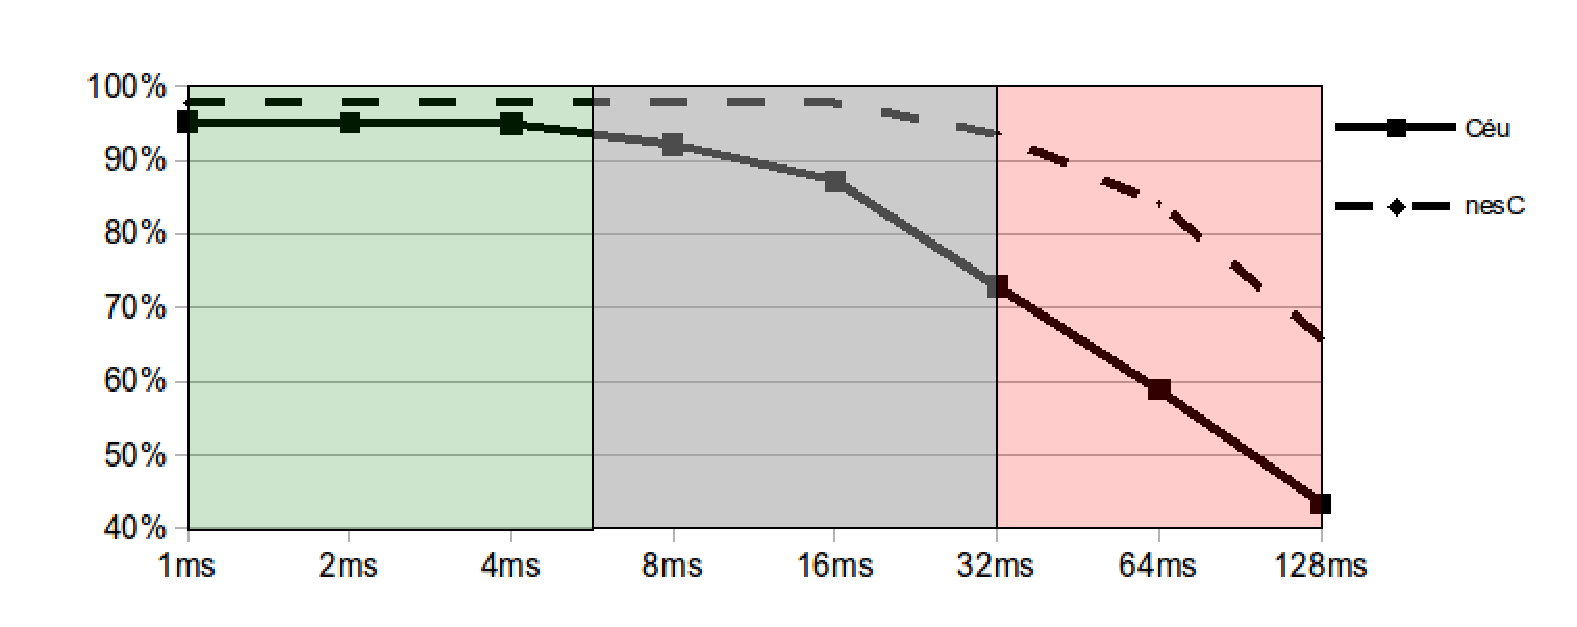
\includegraphics[width=\linewidth,clip=true,trim=35px 0px 10px 0px]{radio1}
\caption{ Percentage of received packets depending on the duration of the 
lengthy operation.  \newline
{\small %\textmd{
Note the logarithmic scale on the \emph{x}-axis.
The packet arrival frequency is 20ms.
The operation frequency is 140ms.
%Starting from a 16-ms duration, \CEU performs 5\% worse than \emph{nesC}.
In the (left) green area, \CEU performs similarly to \emph{nesC}.
The (middle) gray area represents the region in which \emph{nesC} is still 
responsive.
In the (right) red area, both implementations become unresponsive (i.e. over 
5\% packet losses).
}%}
\label{fig.radio1}
}
\end{figure}

\definecolor{lightgreen}{rgb}{.8,1,0.8}
\definecolor{lightred}{rgb}{1,.8,.8}
\definecolor{darkgray}{rgb}{.66,.66,.66}

\begin{table}[t]
\begin{center}
\begin{tabular}{ | l | r | }
\hline
\rowcolor{darkgray}
    Operation          & Duration  \\ \hline
\hline
\rowcolor{lightgreen}
    Block cipher~\cite{wsn.tinysec,wsn.crypto}  & 1ms           \\ \hline
\rowcolor{lightgreen}
    MD5 hash~\cite{wsn.crypto}                  & 3ms           \\ \hline
\rowcolor{lightgreen}
    Wavelet decomposition~\cite{wsn.wavelet}    & 6ms           \\ \hline
\hline
\rowcolor{lightred}
    SHA-1 hash~\cite{wsn.crypto}                & 8ms           \\ \hline
\rowcolor{lightred}
    RLE compression~\cite{wsn.compression}      & 70ms          \\ \hline
\rowcolor{lightred}
    BWT compression~\cite{wsn.compression}      & 300ms         \\ \hline
\rowcolor{lightred}
    Image processing~\cite{wsn.cyclops}         & 50--1000ms    \\ \hline
\end{tabular}
\caption{Durations for lengthy operations is WSNs. \newline
{\small %\textmd{
\CEU can perform the operations in the green rows in real-time and under high 
loads.
}%}
\label{tab.durs}
}
\end{center}
\end{table}

Although we did not perform specific tests to evaluate CPU usage and battery 
consumption, the experiment suggests that the overhead of \CEU over \emph{nesC} 
is very low.
%
When the radio driver is the only running activity (column $1ms$, which is the 
same result for an addition test we did for $0ms$), both implementations loose 
packets with a difference under 3 percentage points.
This difference remains the same up to 4-ms activities, hence, the observed 
degradation for longer operations is only due to the lack of preemption, not 
execution speed.
%
Note that for lengthy operations implemented in $C$, there is no runtime or 
battery consumption overhead at all, as the generated code is the same for \CEU 
and \emph{nesC}.

In the second experiment, instead of running a long activity in parallel, we 
use a 8-ms operation tied in sequence with every packet arrival to simulate an 
activity such as encryption.
We now run the experiment varying the rate in the 10 sending motes from 600ms 
to 100ms (i.e., 60ms to 10ms receiving rate if we consider the 10 motes).
%
Figure~\ref{fig.radio2} shows the percentage of handled packets in \CEU and 
\emph{nesC} for each rate of message arrival.
%
%The last column shows the theoretical limit of 80ms (i.e., receiving a packet 
%every 8ms and handling it in 8ms).
%
The results show that \CEU is 100\% responsive up to frequency of 33 packets 
per second, while \emph{nesC} up to 50 packets.

\begin{figure}[t]
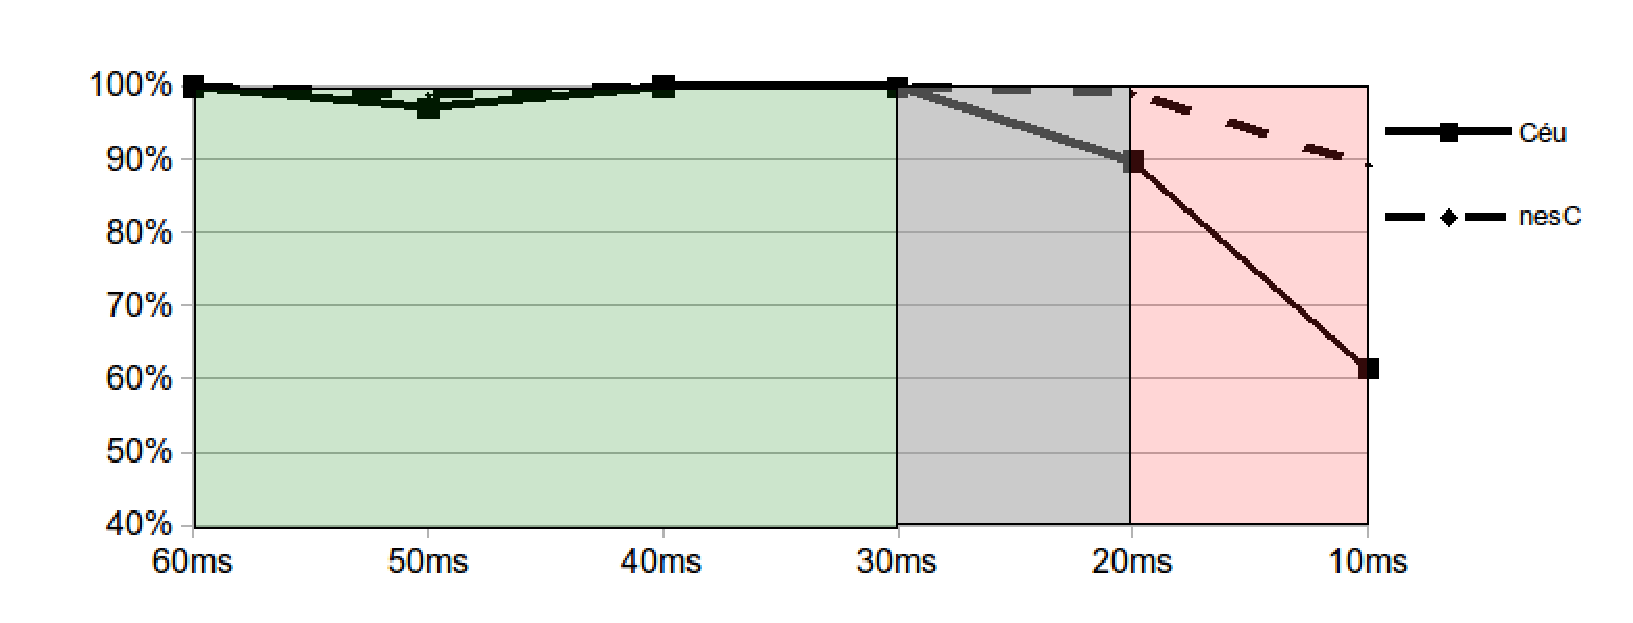
\includegraphics[width=\linewidth,clip=true,trim=35px 0px 10px 0px]{radio2}
\caption{  Percentage of received packets depending on the sending frequency.  
\newline
{\small %\textmd{
Each received packet is tied to a 8-ms operation.
\CEU is 100\% responsive up to a frequency of 30ms per packet.
}%}
\label{fig.radio2}
}
\end{figure}

% TODO: reaction times, measure or cite?

The overall conclusion from the experiments is that the radio driver in \CEU 
performs as well as the original driver in \emph{nesC} under high loads for 
programs with lengthy operations of up to 4ms, which is a reasonable time for 
control execution and simple processing.
%
The range between 6ms and 16ms offers opportunities for performing more complex 
operations, but also requires careful analysis and testing.
%
For instance, the last experiment shows that the \CEU driver can process in 
real time messages arriving every 33ms in sequence with a 8-ms operation.
%
%For operations over 64ms, neither \CEU or \emph{nesC} have real-time 
%responsiveness under high-loads.

Note that our experiments represent a ``stress-test'' scenario that is atypical 
to WSNs.
Protocols commonly use longer intervals between message transmissions together 
with mechanisms to avoid contention, such as randomized 
timers \cite{wsn.trickle,wsn.ctp}.
Furthermore, WSNs are not subject to strict deadlines, being not classified as 
hard real-time systems~\cite{wsn.decade}.

\subsection{Discussion}

\CEU targets control-intensive applications and provides abstractions that can 
express program flow specifications concisely.
%
Our evaluation shows a considerable decrease in code size that comes from 
logical compositions of trails through the \code{par/or} and \code{par/and} 
constructs.
%
They handle start-up and termination for trails seamlessly without extra 
programming efforts.
%
We believe that the small overhead in memory qualifies \CEU as a realistic 
option for constrained devices.
%
% TODO:
%Support for local variables did not lead to reduction in RAM, they and
%are and increase .
%
% TODO
%with overheads below 5\% and 10\%
%Some overhead in memory exists, but RAM is minimal and can be avoided XXX an 
%trackable
%inherent per-trail overhead.
%
%The overhead in ROM is below 10\% but has not .
%
%The main aspect of \CEU is to ensure that the high degree of concurrency in 
%WSNs does not pose safety threats to applications.
%
Furthermore, our broad safety analysis, encompassing all proposed concurrency 
mechanisms, ensures that the high degree of concurrency in WSNs does not pose 
safety threats to applications.
%
%Even with the restrictions that were needed to enable this analysis, \CEU was 
%shown to be expressive enough to imply in a decrease in code complexity for a 
%range of typical WSN applications.
%
%By restricting the expressiveness of the language, we could enable a broad 
%safety analysis in programs at compile time.
%The analysis encompasses all proposed concurrency mechanisms, such as parallel 
%compositions, first-class timers, and communication via events.
%
As a summary, the following safety properties hold for all programs that 
successfully compile in \CEU:

\begin{itemize}
\item Time-bounded reactions to the environment
        (Sections \ref{sec.ceu.det} and \ref{sec.ceu.ints}).
\item Reliable weak and strong abortion among activities
        (Sections~\ref{sec.ceu.det} and \ref{sec.ceu.shared}).
\item No concurrency in accesses to shared variables
(Section~\ref{sec.ceu.shared}).
\item No concurrency in system calls sharing a resource
        (Section~\ref{sec.ceu.c}).
\item Finalization for blocks going out of scope
        (Section~\ref{sec.ceu.fins}).
\item Auto-adjustment for timers in sequence
        (Section~\ref{sec.ceu.wclocks}).
\item Synchronization for timers in parallel
        (Section~\ref{sec.ceu.wclocks}).
\end{itemize}

These properties are desirable in any application and are guaranteed as 
preconditions in \CEU by design.
Ensuring or even extracting these properties from less restricted languages 
requires significant manual analysis.

Even though the achieved expressiveness and overhead of \CEU meet the 
requirements of WSNs, its design imposes two inherent limitations:
the lack of dynamic loading which would forbid the static analysis,
and the lack of hard real-time guarantees.

Regarding the first limitation, dynamic features are already discouraged due to 
resource constraints.
For instance, even object-oriented languages targeting WSNs forbid dynamic 
allocation~\cite{wsn.flowtalk,wsn.virgil}.
%
Given that we focus on system-level development which does not require rich 
dynamic functionality, we leave for a future work an in-depth discussion about 
this issue.
Note that queues, stacks, and other simple dynamic data structures for handling 
message packets can be made available to \CEU through its safe integration with 
$C$.

To deal with the second limitation, which can be critical in the presence of 
lengthy computations, we can consider the following approaches:
(1) manually placing \code{pause} statements in unbounded loops;
(2) integrating \CEU with a preemptive system.
%
The first option requires the lengthy operations to be rewritten in \CEU using
\code{pause} statements so that other trails can be interleaved with them.
This option is the one recommended in many related work that provide a similar 
cooperative primitive (e.g. \code{pause}~\cite{esterel.primer}, 
\code{PT\_YIELD}~\cite{wsn.protothreads}, \code{yield}~\cite{wsn.sol}, 
\code{post}~\cite{wsn.nesc}).
%
Considering the second option, \CEU and preemptive threads are not mutually 
exclusive.
% and the second option is appealing to be explored in a future work.
For instance, TOSThreads~\cite{wsn.tosthreads} proposes a message-based 
integration with \emph{nesC} that is safe and matches the semantics of \CEU 
external events.

\section{Related Work}
\label{sec.related}

\begin{figure*}[t]
\includegraphics[width=\textwidth,clip=true,trim=110px 340px 120px 0px]{related}
\caption{ Table of features found work related to \CEU. \newline
{\small %\textmd{
The languages are sorted by the date they first appeared in a publication.
A gray background indicates where the feature first appeared (or a contribution 
if it appears in a \CEU cell).
}%}
\label{fig.related}
}
\end{figure*}

\CEU is strongly influenced by Esterel~\cite{esterel.ieee91} in its support for 
compositions and reactivity to events.
However, Esterel is focused only on control and delegates to programmers most 
efforts to deal with data and low-level access to the underlying platform.
For instance, read/write to shared memory among threads is forbidden, and 
avoiding conflicts between concurrent $C$ calls is left to 
programmers~\cite{esterel.primer}.
\CEU deals with shared memory and $C$ integration at its very core, with 
additional support for finalization, conflict annotations, and a static 
analysis that permeates all languages aspects.
This way, \CEU could not be designed easily as pure extensions to Esterel.

Figure~\ref{fig.related} presents an overview of work related to \CEU, pointing 
out supported features which are grouped by those that reduce complexity and 
those that increase safety.
The line \emph{Preemptive} represents languages with preemptive 
scheduling~\cite{wsn.mantisos,wsn.tosthreads}, which are summarized further.
The remaining lines enumerate languages with goals similar to those of \CEU 
that follow a synchronous or cooperative execution semantics.

Many related approaches allow events to be handled in sequence through a 
blocking primitive, overcoming the main limitation of event-driven systems 
(column~1~\cite{wsn.protothreads, wsn.ocram, wsn.tinythreads, wsn.flowtalk, 
wsn.sol}).
%
As a natural extension, most of them also keep the state of local variables 
between reactions to the environment (column~2).
In addition, \CEU introduces a reliable mechanism to interface local pointers 
with the system through finalization blocks (column~8).
%, as discussed in Section~\ref{sec.ceu.fins}.
%
Given that these approaches use cooperative scheduling, they can provide 
deterministic and reproducible execution (column~5).
%
However, as far as we know, \CEU is the first system to extend this guarantee 
for timers in parallel.

Synchronous languages first appeared in the context of WSNs through 
OSM~\cite{wsn.osm} and Sol~\cite{wsn.sol}, which provide parallel compositions 
(column~3) and distinguish themselves from multi-threaded languages by handling 
thread destruction seamlessly~\cite{sync_async.threadsstop,esterel.preemption}.
Compositions are fundamental for the simpler reasoning about control that made 
possible the safety analysis of \CEU.
%
Sol detects infinite loops at compile time to ensure that programs are 
responsive (column~6).
\CEU adopts the same policy, which first appeared in Esterel.
%
Internal events (column~4) can be used as a reactive alternative to 
shared-memory communication in synchronous languages, as supported in OSM.
\CEU introduces a stack-based execution that also provides a restricted but 
safer form of subroutines.
% (as discussed in Section~\ref{sec.ceu.ints}).

\emph{nesC} provides a data-race detector for interrupt handlers (column~7), 
ensuring that \emph{``if a variable x is accessed by asynchronous code, then 
any access of x outside of an atomic statement is a compile-time 
error''}~\cite{wsn.nesc}.
The analysis of \CEU is, instead, targeted at synchronous code and points more 
precisely when accesses can be concurrent, which is only possible because of 
its restricted semantics.
Furthermore, \CEU extends the analysis for system calls (\emph{commands} in 
\emph{nesC}), as well as conflicts in trail termination.
Although \emph{nesC} does not enforce bounded reactions, it promotes a 
cooperative style among tasks, and provides asynchronous events that can 
preempt tasks (column 6), something that cannot be done in \CEU.
% (as discussed in Sections~\ref{sec.ceu.det} and \ref{sec.ceu.c}).

On the opposite side of concurrency models, languages with preemptive 
scheduling assume time independence among processes and are more appropriate 
for applications involving algorithmic-intensive problems.
%
Preemptive scheduling is also employed in real-time operating systems to 
provide response predictability, typically through prioritized schedulers
~\cite{wsn.mantisos,wsn.oses,freertos,wsn.tosthreads}.
%
The choice between the two models should take into account the nature of the 
application and consider the trade-off between safe synchronization and 
predictable responsiveness.

\section{Conclusion}
\label{sec.conclusion}

% TTT: corroborar results dos outros trabalhos

We presented \CEU, a system-level programming language targeting 
control-intensive WSN applications.
\CEU is based on a synchronous core that combines parallel compositions with 
standard imperative primitives, such as sequences, loops and assignments.
%
Our work has three main contributions:
%
\begin{itemize}
%
\item A resource-efficient synchronous language that can express control 
      specifications concisely.
%
\item The stack-based execution policy for internal events as a powerful 
      broadcast communication mechanism.
%
\item A wide set of compile-time safety guarantees for concurrent programs that 
      are still allowed to share memory and access the underlying platform in 
``raw $C$''.
%
\end{itemize}
%
We argue that the dictated safety mindset of our design does not lead to a 
tedious and bureaucratic programming experience.
%
In fact, the proposed safety analysis actually depends on control information 
that can only be inferred based on high-level control-flow mechanisms (which 
results in more compact implementations).
%
Furthermore, \CEU embraces practical aspects for the context of WSNs, providing 
seamless integration with $C$ and a convenient syntax for timers.
%
%This relationship between safety and expressiveness is two-way, and
%also rely on the safety guarantees to be trustworthy.

As far as we know, \CEU is the first language with stack-based internal events, 
which allows to build rich control mechanisms on top of it, such as a limited 
form of subroutines and exception handling.
%
In particular, \CEU's subroutines compose well with the other control 
primitives and are safe, with guaranteed bounded execution and memory 
consumption.

Our evaluation compares several implementations of widely adopted WSN protocols 
in \CEU to \emph{nesC}, showing a considerable reduction in code size with a 
small increase in resource usage.
%
On the way to a more in-depth qualitative approach, we have been teaching \CEU 
as an alternative to \emph{nesC} in hands-on WSN courses in a high school for 
the past two years (and also in two universities in short courses).
Our experience shows that students are capable of implementing a simple 
multi-hop communication protocol in \CEU in a couple of weeks.

The resource-efficient implementation of \CEU is suitable for constrained 
sensor nodes and imposes a small memory overhead in comparison to handcrafted 
event-driven code.

%TODO
%The simpler static analysis executes in negligible time for all 
%implementations to be presented in Section~\ref{sec.eval} and does not detect 
%any false positives, suggesting that the algorithm is practical.

\section{Acknowledgments}

This work was partially supported by grants from CNPq (Brazil), SAAB (Sweden), 
and the European Union Seventh Framework Programme (FP7/2007-2013) under 
agreement No. 257007.

%\newpage % TTT
\balance
%{\footnotesize
\bibliographystyle{abbrv}
\bibliography{other}
%}

\end{document}
